\section{Relaying between neighboring cubes}\label{sec:geometry}

The contraction and translation strategy adapts the quarter-face targets
of Kozma and Nitzan~\cite[Section~4, Lemmas~11--12]{KozmaNitzan2024}.
We specify thirteen moves that turn the extension estimate into a connection
estimate between the present neighboring coarse boxes. The scales $R,r$ and the parameter $q$ are those of
Lemma~\ref{prelim:scales}; in particular,
\begin{equation}\label{geom:separation}
  r>100(R+1).
\end{equation}
For $v=(v_1,v_2)\in\mathbb Z^2$, set
\begin{equation}\label{geom:boxes}
  c_v=(20r+1)(v_1,v_2,0),\qquad
  Q_v=\Lambda_{10r}(c_v),\qquad
  B_v=\Lambda_{4r}(c_v).
\end{equation}
The cubes $Q_v$ have disjoint vertex sets. If $v,x$ are nearest neighbors in
$\mathbb Z^2$, let $I_{vx}$ be the set of lattice edges with one endpoint in
$Q_v$ and the other in $Q_x$. Their union $D=Q_v\cup Q_x$ is a rectangular
lattice prism: all edges internal to $D$ are precisely the edges internal to
the two cubes together with $I_{vx}$.

\begin{lemma}[Neighboring-box relay]\label{geom:relay}
Let $v,x\in\mathbb Z^2$ be nearest neighbors. Let $G$ be a finite lattice
subgraph containing $D=Q_v\cup Q_x$ and all lattice edges internal to $D$.
Consider independent bond or site percolation on $G$, with parameter $q$ on
all bits internal to $D$ and arbitrary parameters elsewhere. If $o\in V(G)$
lies outside $D$, then
\begin{equation}\label{geom:relay-bound}
  \mathbb P\bigl(o\leftrightarrow B_v,\ o\not\leftrightarrow B_x\bigr)
  \le 13\eta.
\end{equation}
All connections in this statement are taken in $G$.
\end{lemma}

\begin{proof}
By translation and a signed permutation of coordinates, we may suppose that
$c_v=0$ and $c_x=(20r+1,0,0)$. Thus
\begin{equation}\label{geom:prism}
  D=\bigl([-10r,30r+1]\times[-10r,10r]^2\bigr)\cap\mathbb Z^3.
\end{equation}
Indeed, the first-coordinate intervals of the two cubes are
$[-10r,10r]\cap\mathbb Z$ and $[10r+1,30r+1]\cap\mathbb Z$, whose union has
no missing lattice vertices.

We construct rectangles $P_0,\ldots,P_{13}$, starting with $P_0=B_v$ and
ending with $P_{13}\subseteq B_x$, such that
Lemma~\ref{ext:estimate} applies with $B=P_i$ and $T=P_{i+1}$ for every
$0\le i<13$. At each translation, the required $R$-expansion of the starting
rectangle is accommodated by increasing every half-width by $R$.
We first shorten the rectangle in each of its three coordinate directions,
leaving room for ten such increases before the final rectangle must fit
inside $B_x$. Figure~\ref{geom:figure} shows these two stages, and
Table~\ref{geom:interfaces} records the thirteen target rectangles and
the radii and orientations used to choose the quarter-faces.

\begin{figure}[tbp]
\centering
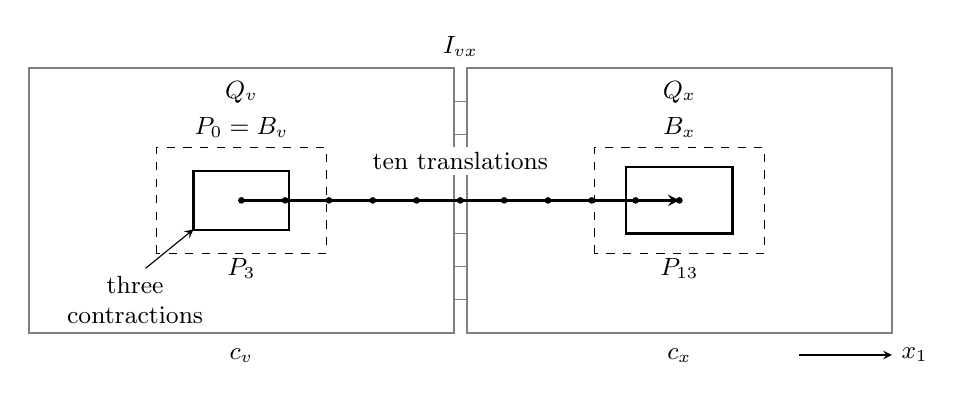
\begin{tikzpicture}[x=1.35cm,y=1.05cm,font=\small,>=stealth]
  \draw[gray,thick] (0,0) rectangle (4,3.2);
  \draw[gray,thick] (4.12,0) rectangle (8.12,3.2);
  \node at (2,2.91) {$Q_v$};
  \node at (6.12,2.91) {$Q_x$};
  \foreach \y in {0.4,0.8,1.2,1.6,2.0,2.4,2.8}{
    \draw[gray] (4,\y)--(4.12,\y);
  }
  \node[above] at (4.06,3.22) {$I_{vx}$};
  \draw[dashed] (1.2,0.96) rectangle (2.8,2.24);
  \draw[dashed] (5.32,0.96) rectangle (6.92,2.24);
  \node at (2,2.48) {$P_0=B_v$};
  \node at (6.12,2.48) {$B_x$};
  \draw[thick] (1.55,1.24) rectangle (2.45,1.96);
  \draw[thick] (5.62,1.20) rectangle (6.62,2.00);
  \node at (2,0.78) {$P_3$};
  \node at (6.12,0.78) {$P_{13}$};
  \draw[->,thick] (2,1.6)--(6.12,1.6);
  \foreach \i in {0,...,10}{
    \fill ({2+0.412*\i},1.6) circle (1.2pt);
  }
  \node[fill=white,inner sep=2pt] at (4.06,2.08) {ten translations};
  \draw[->] (1.1,0.78)--(1.55,1.25);
  \node[align=center] at (1.0,0.40) {three\\contractions};
  \node[below] at (2,-0.08) {$c_v$};
  \node[below] at (6.12,-0.08) {$c_x$};
  \draw[->] (7.25,-0.27)--(8.12,-0.27) node[right] {$x_1$};
\end{tikzpicture}
\caption{A schematic cross-section of the neighboring-box relay, not to scale.
The three contraction steps take $P_0$ to $P_3$; the marked centers then make
ten translations to $P_{13}\subset B_x$. Intermediate rectangles are omitted.
The last translation has length $2r+1$, rather than $2r$, to match the coarse
spacing $20r+1$. The narrow gap represents the interface edges between disjoint
lattice cubes, not a missing layer of lattice vertices.}
\label{geom:figure}
\end{figure}

\begin{table}[tbp]
\centering
\small
\begin{tabular}{c c c c c}
\hline
Target & Center's first coordinate & Coordinate half-widths & Radius & Normal\\
\hline
$P_1$ & $0$ & $(2r+R,4r+R,4r+R)$ & $2r$ & $1$, inward\\
$P_2$ & $0$ & $(2r+2R,2r+2R,4r+2R)$ & $2r$ & $2$, inward\\
$P_3$ & $0$ & $(2r+3R,2r+3R,2r+3R)$ & $2r$ & $3$, inward\\
$P_4$ & $2r$ & $(2r+4R)\mathbf1$ & $2r$ & $1$, forward\\
$P_5$ & $4r$ & $(2r+5R)\mathbf1$ & $2r$ & $1$, forward\\
$P_6$ & $6r$ & $(2r+6R)\mathbf1$ & $2r$ & $1$, forward\\
$P_7$ & $8r$ & $(2r+7R)\mathbf1$ & $2r$ & $1$, forward\\
$P_8$ & $10r$ & $(2r+8R)\mathbf1$ & $2r$ & $1$, forward\\
$P_9$ & $12r$ & $(2r+9R)\mathbf1$ & $2r$ & $1$, forward\\
$P_{10}$ & $14r$ & $(2r+10R)\mathbf1$ & $2r$ & $1$, forward\\
$P_{11}$ & $16r$ & $(2r+11R)\mathbf1$ & $2r$ & $1$, forward\\
$P_{12}$ & $18r$ & $(2r+12R)\mathbf1$ & $2r$ & $1$, forward\\
$P_{13}$ & $20r+1$ & $(2r+13R)\mathbf1$ & $2r+1$ & $1$, forward\\
\hline
\end{tabular}
\caption{The thirteen interfaces $P_{j-1}\to P_j$ in the relay.
All centers have second and third coordinates zero, and
$\mathbf1=(1,1,1)$. Each listed radius is used about every point
of $P_{j-1}^{(R)}$. ``Inward'' means toward zero in that normal coordinate;
``forward'' means the positive first direction. All transverse signs point
toward zero. The proof verifies both target-face and full-cube containment.}
\label{geom:interfaces}
\end{table}

\paragraph{Three contraction steps.}
For $t=1,2,3$, let $P_t$ be centered at zero with coordinate half-widths
\begin{equation}\label{geom:contraction-widths}
  a_{t,h}=\begin{cases}
    2r+tR,&h\le t,\\
    4r+tR,&h>t,
  \end{cases}
  \qquad h\in\{1,2,3\}.
\end{equation}
Fix $u\in P_{t-1}^{(R)}$. Its coordinate bounds are $2r+tR$ in directions
$h<t$ and $4r+tR$ in directions $h\ge t$. In the cube $\Lambda_{2r}(u)$,
choose a quarter-face normal to coordinate $t$, with its normal sign and both
transverse signs directed toward coordinate zero. At a zero coordinate,
either sign may be used.

In the normal direction, the face coordinate has absolute value at most
\[
  \max\{2r,(4r+tR)-2r\}=2r+tR.
\]
In a transverse direction, the face coordinate ranges between a number $a$
and $a-2r\operatorname{sign}(a)$, with either sign allowed when $a=0$.
Its absolute value is therefore at most $\max\{|a|,2r\}$, which fits the
corresponding half-width in \eqref{geom:contraction-widths}. The chosen
quarter-face is consequently contained in $P_t$.

The full cube $\Lambda_{2r}(u)$ has all coordinate absolute values at most
$6r+3R<10r$, by \eqref{geom:separation}, and so lies in $D$. In particular
$P_{t-1}^{(R)}\subseteq D$. Since $o\notin D$, the remaining geometric
hypothesis of Lemma~\ref{ext:estimate} is also satisfied. This proves its
applicability to all three contraction steps. The resulting rectangle is
\begin{equation}\label{geom:contracted}
  P_3=\Lambda_{2r+3R}(0).
\end{equation}

\paragraph{Ten translation steps.}
Define the step lengths and centers by
\begin{equation}\label{geom:translations}
  s_i=\begin{cases}2r,&1\le i\le9,\\2r+1,&i=10,\end{cases}
  \qquad
  z_0=0,\qquad z_i=(s_1+\cdots+s_i,0,0).
\end{equation}
For $1\le i\le10$, set
\begin{equation}\label{geom:translated-boxes}
  w_i=2r+(3+i)R,\qquad P_{3+i}=\Lambda_{w_i}(z_i).
\end{equation}
The $R$-expansion of the preceding rectangle, $P_{2+i}^{(R)}$, is centered
at $z_{i-1}$ and has half-width $w_i$. Fix $u$ in that expansion. In
$\Lambda_{s_i}(u)$ choose the quarter-face with forward normal in coordinate
$1$, and with both transverse signs directed toward zero. The normal
coordinate on this face is $u_1+s_i$. Relative to the new center $z_i$, its
offset is exactly $u_1-(z_{i-1})_1$, of absolute value at most $w_i$.
Transverse absolute coordinates are at most
$\max\{w_i,s_i\}=w_i$. The equality also holds for the last step, because
$13R\ge1$. Hence this quarter-face is contained in $P_{3+i}$.

To check containment of the full radius-$s_i$ cube, note that
$0\le(z_{i-1})_1\le18r$, $w_i\le2r+13R$, and $s_i\le2r+1$. Its first
coordinate is therefore between
\begin{equation}\label{geom:translation-bounds}
  -4r-13R-1\quad\hbox{and}\quad22r+13R+1,
\end{equation}
and its transverse absolute coordinates are at most $4r+13R+1$.
Condition~\eqref{geom:separation} gives $13R+1<6r$ and $13R<8r$, so these
bounds lie inside the prism \eqref{geom:prism}. It follows again that the
preceding expanded rectangle lies in $D$ and avoids $o$. The radii used
are $2r$ and $2r+1$, both allowed by Lemma~\ref{ext:estimate}. Thus all ten
translation steps satisfy that Lemma's hypotheses.

The final center is
$z_{10}=(9(2r)+(2r+1),0,0)=c_x$, and the final half-width is
$w_{10}=2r+13R<4r$. Consequently $P_{13}\subseteq B_x$. If $o$ is connected
to $P_0$ but not to $P_{13}$, then for at least one $i\in\{0,\ldots,12\}$
it is connected to $P_i$ but not to $P_{i+1}$. A union bound and thirteen
applications of Lemma~\ref{ext:estimate} now give
\[
\begin{split}
  \mathbb P\bigl(o\leftrightarrow B_v,\ o\not\leftrightarrow B_x\bigr)
  &\le
  \mathbb P\bigl(o\leftrightarrow P_0,\ o\not\leftrightarrow P_{13}\bigr)\\
  &\le \sum_{i=0}^{12}
       \mathbb P\bigl(o\leftrightarrow P_i,\ o\not\leftrightarrow P_{i+1}\bigr)
   \le 13\eta.
\end{split}
\]
No independence between these thirteen connection events is required.
\end{proof}
